% !TEX program = xelatex
\documentclass[letterpaper,11pt]{article}
\usepackage{tabularx} % extra features for tabular environment
\usepackage{amsmath, amssymb, mathtools}  % improve math presentation
\usepackage{graphicx} % takes care of graphics including machinery
\usepackage{url}
\usepackage{chemfig}
\usepackage[version=4]{mhchem}
\usepackage{seqsplit}
\usepackage[margin=2cm,letterpaper]{geometry} % decreases margins
\usepackage{caption}
\usepackage{adjustbox}
\usepackage{booktabs}
\usepackage{cite} % takes care of citations
\usepackage[final]{hyperref} % adds hyperlinks inside the generated pdf file
\hypersetup{
	colorlinks=true,       % false: boxed links; true: colored links
	linkcolor=blue,        % color of internal links
	citecolor=blue,        % color of links to bibliography
	filecolor=magenta,     % color of file links
	urlcolor=blue         
}
\usepackage{blindtext}
\usepackage{amsfonts}
\usepackage{tikz}
\usepackage{standalone}
\usepackage{xcolor}
\usepackage{bookmark}
\usepackage{chemformula}
\usepackage[para]{footmisc}
\usepackage{subcaption}

\setchemfig{atom sep=4em}
\captionsetup{justification=centering, font=small}
\definecolor{darkgray}{gray}{0.3}
\newcommand{\annot}[1]{\textcolor{darkgray}{\textit{#1}}}

\renewcommand{\footnoterule}{%
  \kern-3pt % space above the rule
  \hrule width \textwidth height 0.4pt
  \kern5pt % space below the rule
}

\usepackage{fontspec}
\setmainfont{Arial} % replace 'Arial' with your preferred 

\begin{document}
% TODO: Make the title page centered and in a single page
\title{\vspace{-2em}Evaluation of Differential Expression Profile of Select Genes in Human Fibroblasts Subjected to UV Radiation}
% \vspace{-0.5cm}
\author{Harsh Agrawal (CID - 02320622) \\ Department of Bioengineering, Imperial College London}
\date{}
\maketitle
\vspace{-2em}
\section{Introduction}
UV radiation causes DNA damage by inducing mutagens such as pyrimidine dimers and photoproducts that can lead to mutations in the DNA.\cite{ref:uv_induced_aging_tp53}. This puts the cells in a state of stress, activating various pathways to repair DNA damage, halt the cell cycle, and prevent the formation of cancer. Our aim in this experiment was to evaluate the differential expression profiles of five genes — COL-1, TP53 (personal selection), TERT, MYC, and GAPDH — which are either crucial to cell survival or are part of cell cycle/cell repair pathways in human fibroblasts in response to UV radiation. We also evaluated the methylation status of the promoter regions of two genes — ELOVL2 and COL-1, to understand the epigenetic changes in response to UV radiation. One of the primary motivations for choosing UV as a perturbation source was its direct link to causing DNA mutations, which accumulate to age the cell and can ultimately lead to cancer.

GAPDH (Glyceraldehyde-3-Phosphate Dehydrogenase) is a common `housekeeper gene' that was recently found to play an active role in DNA repair, independent of its glycolytic function. Different studies show varying expression trends of GAPDH in response to aging, while some report no significant change in expression~\cite{ref:gapdh}. Similarly, the COL-1 gene is also a housekeeper gene that encodes for collagen type 1—the most abundant skin protein. The levels of COL-1 are known to decrease with age, leading to the accumulation of degraded collagen in the skin~\cite{ref:col_1}.

\begin{figure}[!ht]
    \centering
    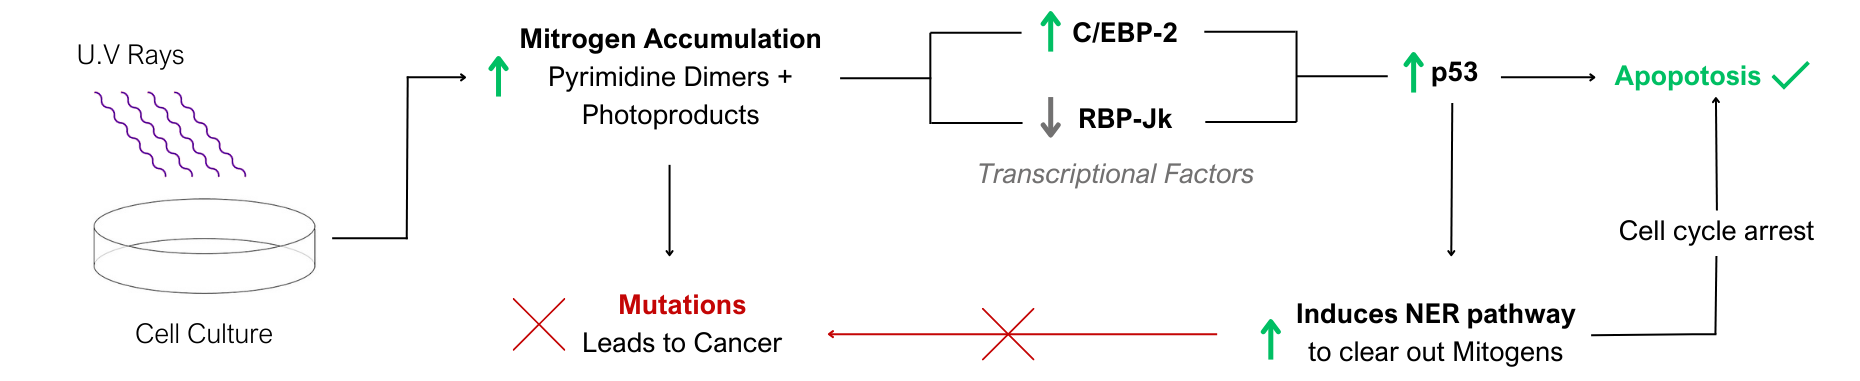
\includegraphics[width=\textwidth]{figures/tp53.png} % first figure
    \caption{Flowchart explaining how p53 prevents accumulation of mutations}\label{fig:tp53}
\end{figure}

TP53 (or p53) is a tumor suppressor gene and is also one of the most studied human genes. It is responsible for inducing cell-cycle arrest via the pathway explained in Figure~\ref{fig:tp53}\cite{ref:tp53_new}. The concentration of TP53 in healthy cells is typically low due to its short half-life. These levels are reportedly elevated by up to ten times in response to UV-induced stress and the urgency to halt cell replication.

TERT (telomerase reverse transcriptase) is an enzyme responsible for maintaining the length of telomeres in DNA. In aged cells, the expression of TERT is found to be greatly decreased, leading to the shortening of telomeres and ultimately cell death\cite{ref:tert}. MYC, on the other hand, promotes gene expression by activating pro-proliferating genes. Its levels are also reportedly found to decrease with age\cite{ref:myc}. Apart from the upregulation of TP53, we expect to see the downregulation of the other six genes in response to aging according to the literature. We also expect the downregulated genes to be hypermethylated and vice versa.

\newpage
\section{Methods}
The initial phase of the experiment involved culturing human fibroblast cells, which were incubated at $37^{\circ}$C with 5\% \ce{CO2} in a medium comprising low glucose DMEM\footnote{DMEM = Dulbecco's Modified Eagle Medium}, 10\% FBS\footnote{FBS = Fetal Bovine Serum}, and 1\% PenStrep\footnote{PenStrep = Penicillin + Streptomycin}. The cells were maintained in a T-25 flask. Subsequently, the cells were passaged (using 1x Trypsin for detachment) and seeded in a 6-well plate at a density of 6000 cells/cm$^2$, at $37^{\circ}$C and 5\% \ce{CO2}. A hemocytometer was employed to count the cells and verify the correct seeding density. Three wells were designated as control and three as UV.

After incubation, the UV wells received 40 mJ/cm$^2$ of UV-A radiation for a minute, were passaged, and incubated again under identical conditions. These cell cultures were then utilized for RNA extraction and Bisulfite sequencing. To begin RNA extraction, cell colonies were first scraped off using an RTL buffer and transferred to separate microcentrifuge tubes. Next, the cells were lysed using the Qiagen QiaShredder. The subsequent step involved removing genomic DNA by adhering to the gDNA Eliminator spin column protocol. Ethanol was then added to the collection from the gDNA spin column to precipitate the RNA. Several rounds of buffer washes in RNeasy spin columns were performed to eliminate contaminants, and purified RNA was ultimately eluted in RNase-free water.

For analyzing various RNA expressions, reverse transcription was performed to synthesize cDNA, followed by PCR amplification. This process was facilitated using a reaction mix prepared with SSIV buffer, DTTs, RNase inhibitor, and the reverse transcriptase enzyme. The necessary volume of RNA was determined by measuring RNA concentration using a Nanodrop spectrophotometer. The derived cDNA was then applied to conduct PCR for five genes, including two caretaker genes — COL-1, GAPDH — and three other genes of interest - TP53, TERT, and MYC. For each gene, three PCR reactions were set up — Control, UV, and \ce{H2O} — totaling 15 PCR reactions. The Platinum II Hot-Start PCR Master Mix was used for these reactions. The primers employed, along with their annealing temperatures, are detailed in Table~\ref{tab:primers}. Primer sequences for TP53, TERT, and MYC were devised by our group, with annealing temperatures, self-complementarity, and product sizes validated using the Oligo Calc tool\footnote{http://biotools.nubic.northwestern.edu/OligoCalc.html}.

PCR products were assessed via Gel Electrophoresis (2g Agarose in 130mL 1x TAE) for 30 minutes at 180V. A 1-Kb ladder from Thermo Fisher served for analysis. Results were visualized under UV light, and images were captured. The band sizes were then compared to the ladder to deduce the genes' expression levels.

Bisulfite Sequencing was undertaken to ascertain methylation patterns in the promoter regions of the \textbf{ELOVL-2} and \textbf{COL-1} genes for both control and UV-treated samples. The bisulfite-modified sequences were aligned and scrutinized for methylation status using CodonCode Aligner\footnote{https://www.codoncode.com/aligner/}.

\begin{table}[!ht]
    \centering
    \footnotesize
    \begin{tabular}{p{1.8cm}p{5.0cm}p{5.2cm}p{2cm}p{1.2cm}}
        \midrule
        Gene                   & Forward Primer                     & Reverse Primer                      & Annealing Temp. ({$^\circ$}C) & Product Size \\
        \midrule
        COL-1                  & ATCACCTGCGTACAGAACGG               & CTGTGTCCCTTCATTCCAGG                & 55.5                          & 712 bp       \\
        \seqsplit{COL-1 (M)}   & \seqsplit{GGGTAGGGTTTTTTTTTGTTTTT} & \seqsplit{CTAAACCCTAAACATATAAACTC}  & 50.5                          & 388 bp       \\
        MYC                    & TGTACCTGCAGGATCTGAGC               & AGGTGATCCAGACTCTGACC                & 55.5                          & 321 bp       \\
        TP53                   & CAGTCAGATCCTAGCGTCGA               & ACATCTTGTTGAGGGCAGGG                & 55                            & 388 bp       \\
        TERT                   & ATTCGCCATTGTTCACCCCT               & CTTCCGTAAATGCACAGCCA                & 53.84                         & 351 bp       \\
        GAPDH                  & CGTCTTCACCACCATGGAGA               & CGGCCATCACGCCACAGTTT                & 55.5                          & 319 bp       \\
        \seqsplit{ELOVL-2 (M)} & \seqsplit{AGGGGYGTAGGGTAAGTGAG}    & \seqsplit{AAACCCAACTATAAACAAAACCAA} & 57.5                          & 183 bp       \\


        \midrule
    \end{tabular}
    \caption{All primers pairs along with their annealing temperatures and product sizes. COL-1 (M) and ELOVL-2 (M) are primers used for Bisulphite Sequencing. The rest are used for PCR.}\label{tab:primers}
\end{table}%
\newpage
\section{Results}
\begin{figure}[!ht]
    \centering
    \begin{subfigure}{0.5\textwidth}
        \centering
        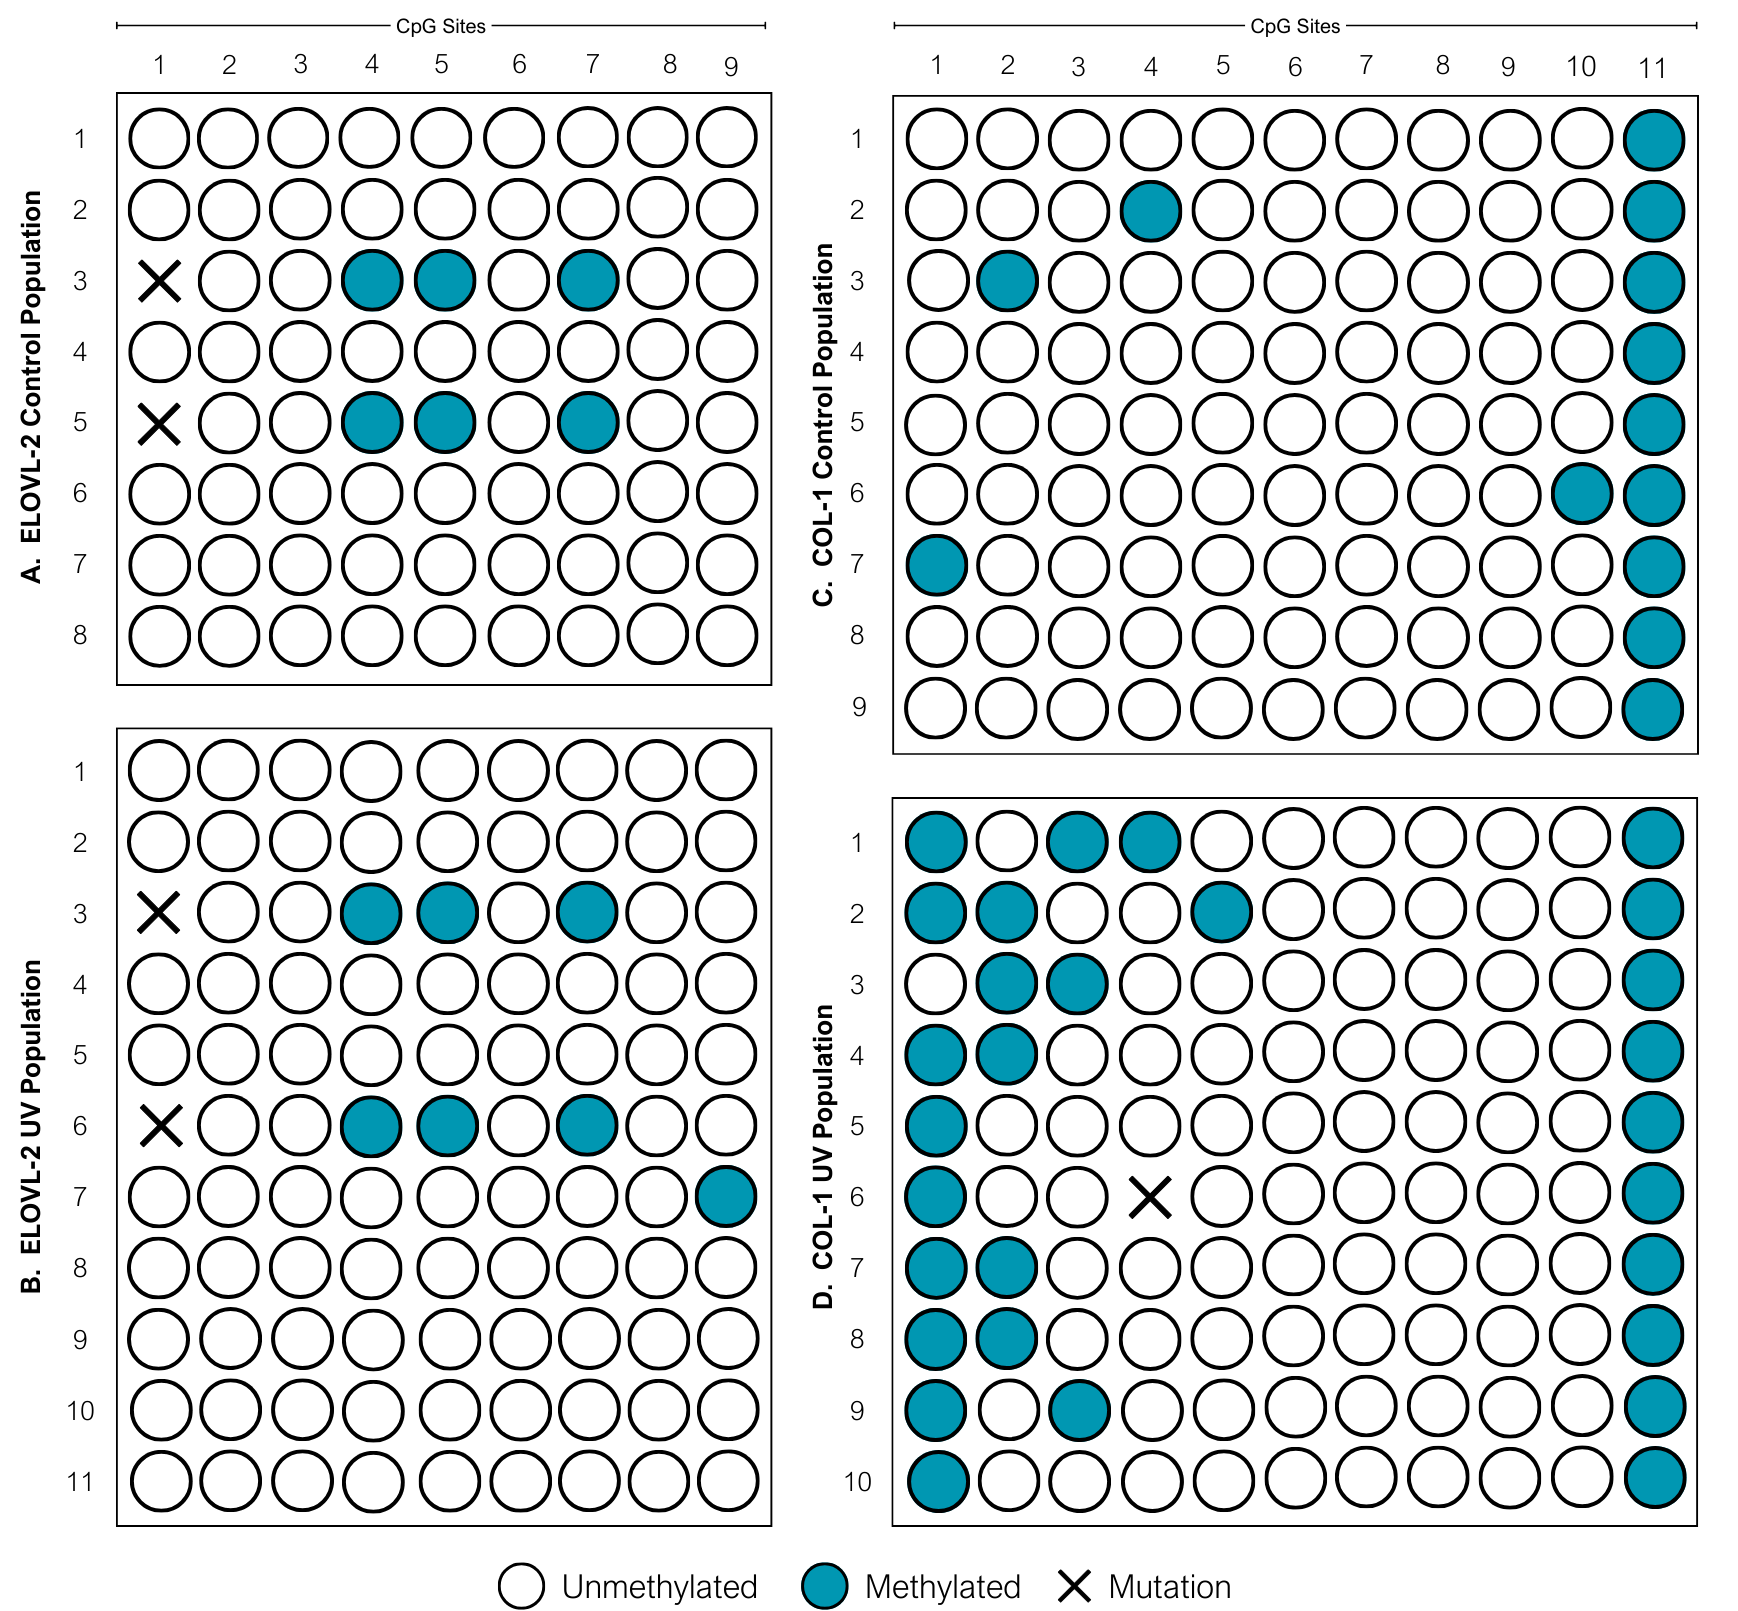
\includegraphics[width=\textwidth]{figures/methylation_data.png} % first figure
        \subcaption{Methylation in promotor regions of ELOVL-2 and COL-1 genes in control and UV samples.}\label{fig:figure1}
    \end{subfigure}\hfill
    \begin{subfigure}{0.5\textwidth}
        \centering
        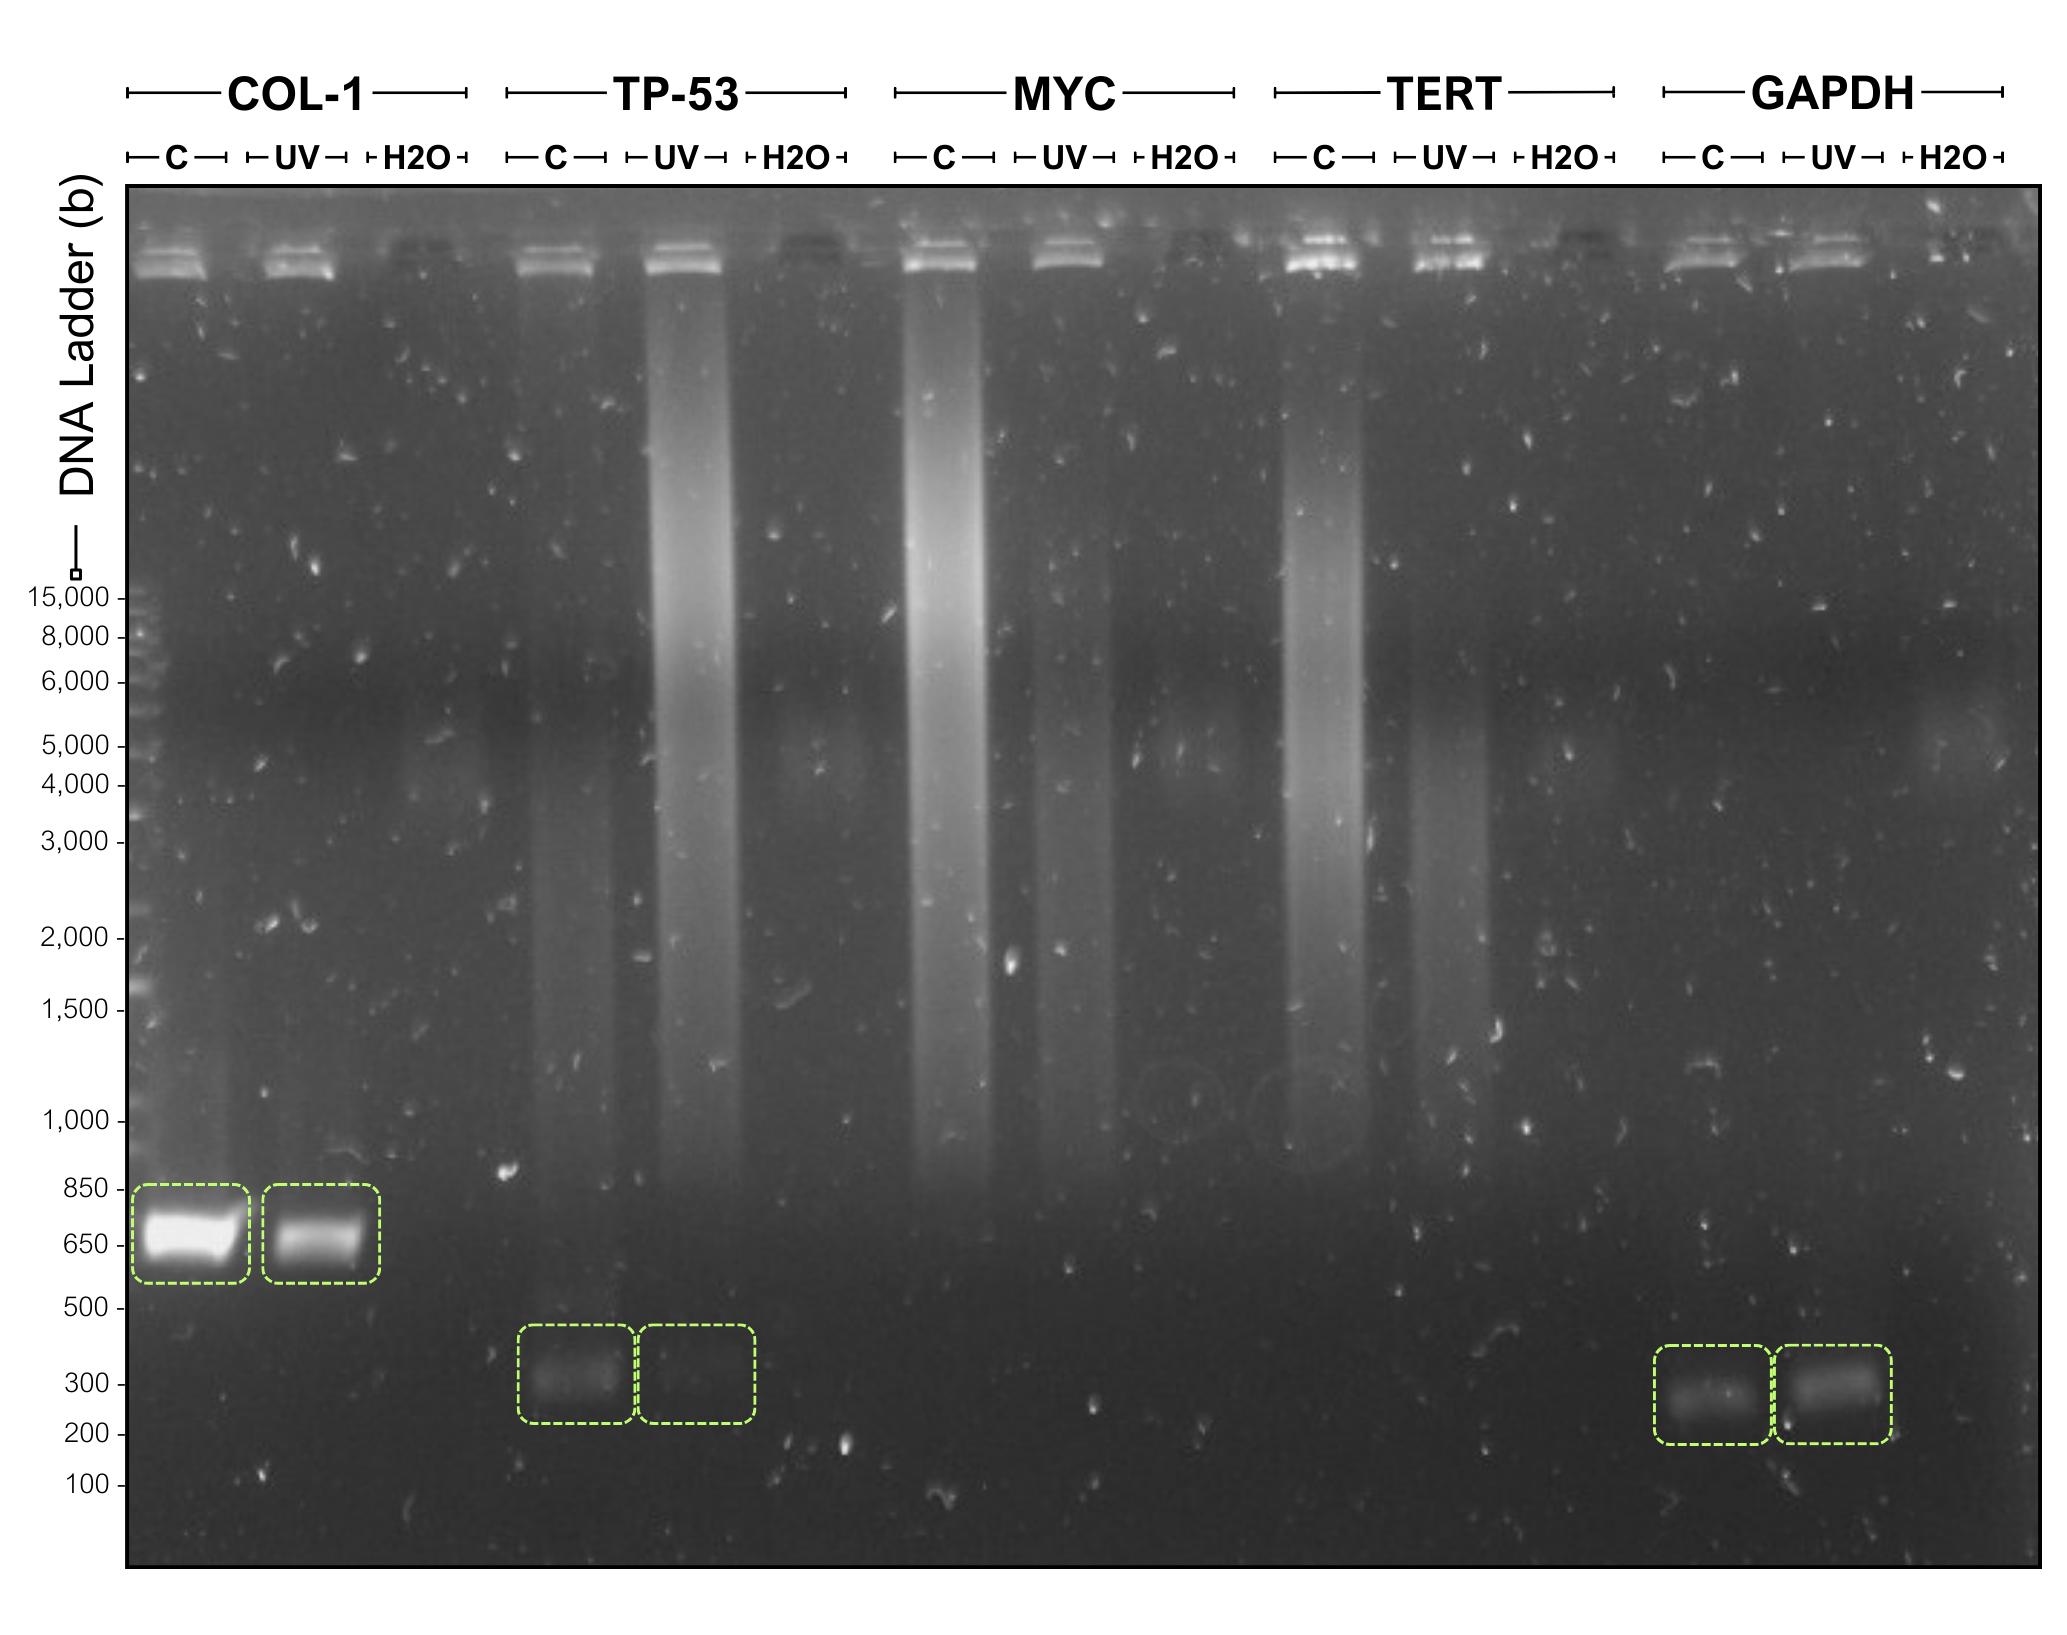
\includegraphics[width=\textwidth]{figures/gel_electrophoresis.png} % second figure
        \subcaption{Gel electrophoresis results for the all five genes (and three samples per gene: UV, control, and $H_{2}O$). A 1-Kb ladder was used from ThermoFisher for analysis.}\label{fig:figure2}
    \end{subfigure}
\end{figure}
The RNA concentration was determined to be 32.88 $ng/\mu L^{-1}$ for control samples compared to 31.64 $ng/\mu L^{-1}$ for UV-treated samples. The A260/A230 and A260/A280 ratios, indicative of contamination, were recorded at 0.4\footnote{Highest purity = 2} and 1.7, respectively. This suggests a satisfactory RNA yield, albeit with substantial contamination likely influencing gene expression outcomes.

Bisulfite sequencing results are depicted in Figure~\ref{fig:figure1}. For the \textbf{ELOVL-2 gene}, the control group showed an average methylation percentage of \textbf{8.3\%} (n\footnote{n = sample size} = 8), while the UV-exposed group had an average of \textbf{7.0\%} (n = 11). An unpaired two-tailed test was applied, yielding a \textbf{p-value = 0.842}. This clearly indicates a lack of statistical significance (p-value > 0.05), demonstrating \textbf{no significant methylation difference} in the promoter region of the ELOVL-2 gene between the control and UV-exposed samples.

In contrast, for the \textbf{COL-1 gene}, the control group's average methylation percentage was \textbf{13.13\%} (n = 9), versus \textbf{26.3\%} in the UV-exposed group (n = 10), with a p-value of \textbf{p < 0.0001}. This highly statistically significant result (p-value < 0.05) suggests that the promoter region of the COL-1 gene is \textbf{hypermethylated} in the UV group compared to the control group.

Gel electrophoresis results of PCR products are illustrated in Figure~\ref{fig:figure2}. The findings reveal that the \textbf{COL-1} gene exhibits a band size of \textbf{approximately 680 bp}, aligning with expected outcomes. The observed brightness differential suggests a \textbf{40--60\% decrease in gene expression} in the UV group. The GAPDH gene's bands do not align with the anticipated product size, indicating potential sample contamination. A pronounced smear was observed in the TP-53, MYC, and TERT genes. In TP-53, bands matching the expected size of 388 bp were identified in both Control and UV groups, with the control band's brightness indicating a \textbf{70--90\% decrease in gene expression}. For MYC and TERT, distinct bands were absent in both control and UV groups, yet the control group's smear brightness was notably higher compared to the UV group, indicating reduced expression in UV-treated samples. A reversed expression trend was noted for TP53.

\newpage
\section{Discussion}
The results provided allow us to definitively assert the downregulation of COL-1 in UV-irradiated samples, corroborated by significant findings of hypermethylation, which inversely correlates with gene expression. Moreover, gel analysis estimates this reduction at approximately 40--50\%, aligning with our initial hypothesis and consistent with other literature findings.

Multiple explanations for the smears observed in TP-53, MYC, and TERT are possible. The presence of distinct bands in COL-1 rules out procedural errors, as all batches underwent identical preparation processes. Additionally, the potential for hairpin structures, self-complementarity, and selective primer binding were all vetted using the Oligo Calc tool. With annealing temperatures standardized across all genes and the base pair lengths set to avoid genomic DNA contamination, the likelihood of gel overload causing the observed smears is minimal, given the absence of fused or distorted bands. This points to the duration of gel running as the probable cause of the issue\cite{ref:gel}. Assuming this to be true, the brightness of the smears could then be indicative of gene expression levels, supporting our initial hypothesis of TP-53 upregulation (evidenced by brighter bands under UV conditions) and MYC and TERT downregulation (indicated by brighter bands in control conditions) in UV-treated samples.

Regarding the ELOVL2 gene, the lack of significant methylation differences between the control and UV groups suggests that UV-induced aging may not impact ELOVL2 expression. The GAPDH results, which showed no intensity difference between control and UV samples, do not provide conclusive insights.

However, it's critical to acknowledge that the conclusions drawn from gel electrophoresis lack statistical significance and accuracy, diminishing confidence in these findings. To answer questions about causality —-- whether TP53 actually induces the NER response or is simply upregulated due to DNA damage —-- other genes in the proposed pathway (e.g., C/EBP-2, EBP-Jk in the TP53 pathway) need to be analyzed, along with performing redundant repeats and including more fibroblast samples.

\bibliographystyle{apalike}
\bibliography{main}
\end{document}
